% This program can be redistributed and/or modified under the terms
% of the GNU Public License, version 3.
%
% Seth Brown, Ph.D.
% sethbrown@drbunsen.org
%
% Compiled with XeLaTeX
% Dependencies:
%   Fontin Sans font (http://www.exljbris.com/fontinsans.html)
%

% TODO: Add citations as bibtex

\documentclass[unknownkeysallowed]{beamer}

\usepackage{graphicx} % graphics
\usepackage{epsfig} % eps graphics
\usepackage{hyperref} % urls
\usepackage{booktabs, caption} % table styling

% suppress navigation bar
\beamertemplatenavigationsymbolsempty

\mode<presentation>
{
  \usetheme{bunsen}
  \setbeamercovered{transparent}
  \setbeamertemplate{items}[circle]
}

% set fonts
\usepackage{fontspec}
\setsansfont{Fontin Sans}
\setbeamerfont{frametitle}{size=\LARGE,series=\bfseries}

% color definitions
\usepackage{color}
\definecolor{uipoppy}{RGB}{225, 64, 5}
\definecolor{uipaleblue}{RGB}{96,123,139}
\definecolor{uiblack}{RGB}{0, 0, 0}

% caption styling
\DeclareCaptionFont{uiblack}{\color{uiblack}}
\DeclareCaptionFont{uipoppy}{\color{uipoppy}}
\captionsetup{labelfont={uipoppy},textfont=uiblack}

% see the macros.tex file for definitions
% This program can be redistributed and/or modified under the terms
% of the GNU Public License, version 3.

% adds reference to bottom right of corner of a slide
\usepackage[absolute,overlay]{textpos} % text references in slide corners
\newcommand\textref[1]{%
  \begin{textblock*}{\paperwidth}(0pt,0.99\textheight)
  \raggedleft \tiny{\emph{#1}}\hspace{.5em}
  \end{textblock*}}

% for drawing circles around numbers
% ex. \circled{1} Add some text here.
\usepackage{tikz}
\newcommand*\circled[1]{\tikz[baseline=(char.base)]{
            \node[shape=circle,draw,inner sep=2pt] (char) {#1};}}


% title slide definition
\title{Get Git}
\author{Chris Keefe, Anthony Simard}
\institute{Northern Arizona University \\
Department of Computer Science \\
School of Informatics, Computing, and Cyber Systems \\
}

\date{\today}

%--------------------------------------------------------------------
%                           Introduction
%--------------------------------------------------------------------

\begin{document}

\section{Introduction}
\setbeamertemplate{background}
{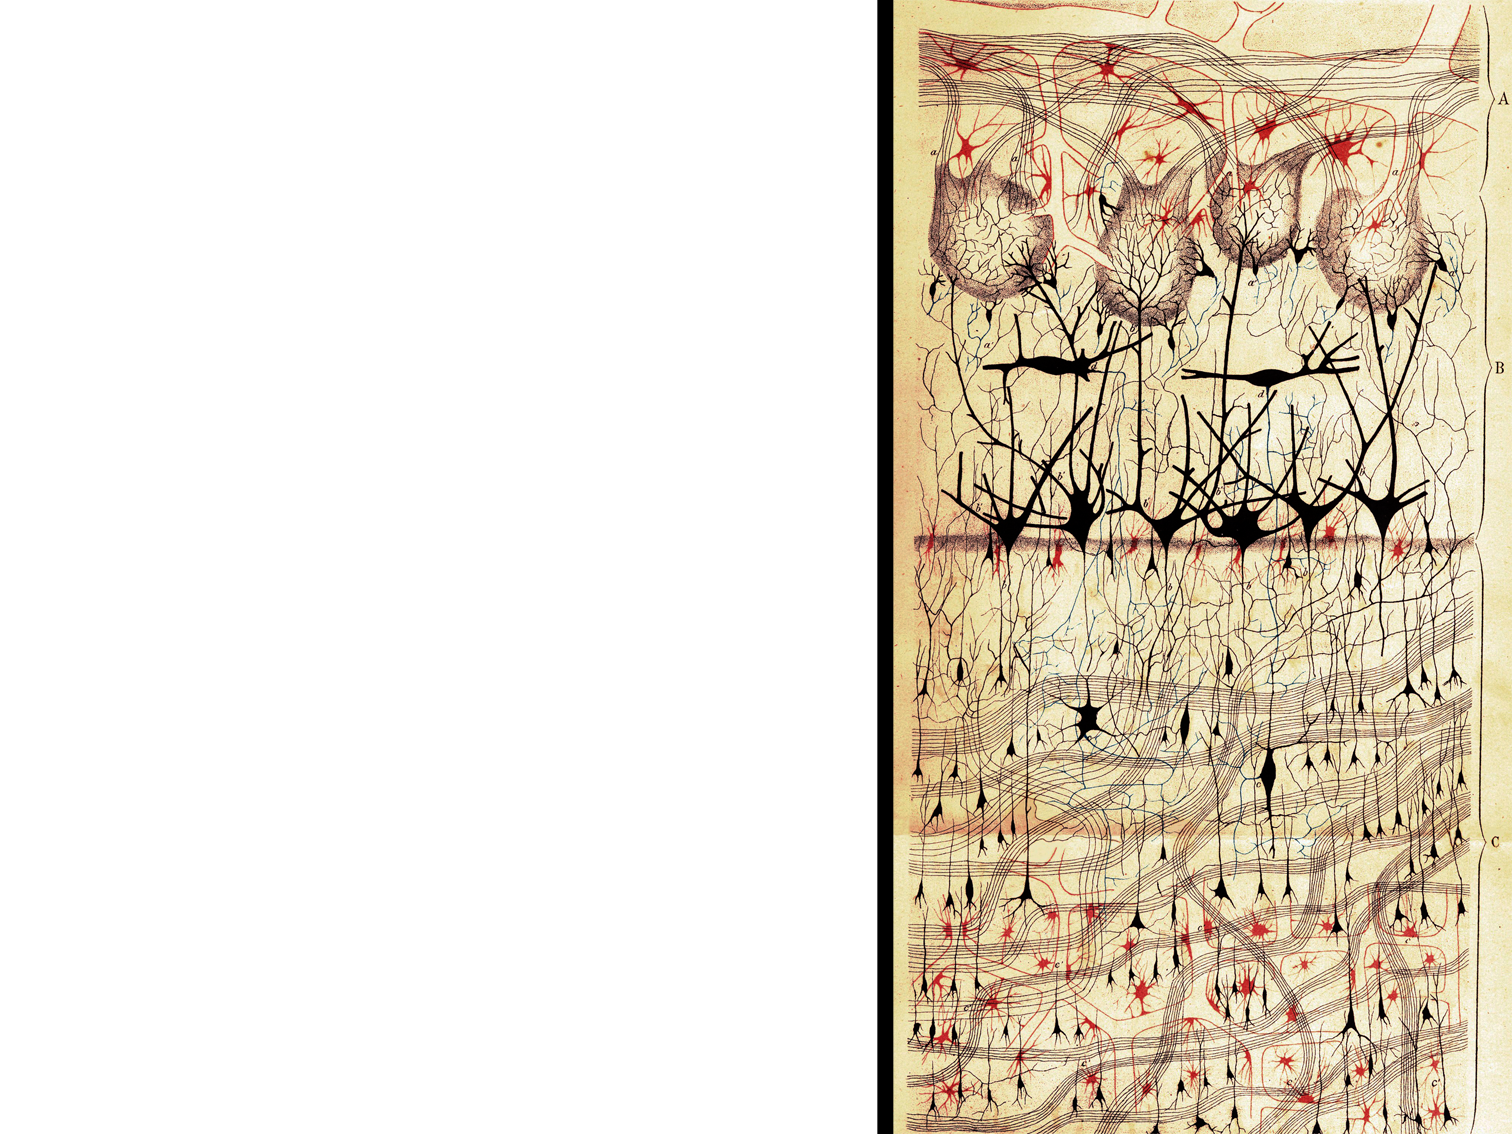
\includegraphics[width=\paperwidth,height=\paperheight]{assets/frontpage_bg}}
\setbeamertemplate{footline}[default]

\begin{frame}
\vspace{2cm}
\begin{columns}
\column{2.75in}
  \titlepage
  \vspace{10cm}
\column{2.0in}
\end{columns}
\end{frame}

%-------------------------------------------------------------------
%                          Section 1
%-------------------------------------------------------------------
%
% Set the background for the rest of the slides.
% Insert infoline
\setbeamertemplate{background}
{
\includegraphics[width=\paperwidth,height=\paperheight]{assets/slide_bg}}
\setbeamertemplate{footline}[bunsentheme]

\section{What, Why, and How?}
\begin{frame}
    \frametitle{What is git?}
    \begin{itemize}
        \item{Git is a powerful version control system}
            \begin{itemize}
                \item{Git allows multiple people to easily update the same source}
                \item{Git makes keeping track of changes easy and robust}
            \end{itemize}
        \item{Git allows people around the world to collaborate on open and closed source projects}
    \end{itemize}
    \vspace{1cm} % generate some space between title and content

    % Keeping all of this for now as an example in case we need to do something like this
    %\begin{table}[h]
    %\centering
    %\begin{tabular}{lcccc} \bottomrule[2pt]
    %    Name & Symbol & $A_r$ & M.P. (K) & IE (J) \\ \bottomrule
    %    Helium & He & $4.00$ & $1$ & $3.94e^{-18}$ \\
    %    Carbon & C & $12.01$ & $773$ & $3.94e^{-18}$ \\
    %    Arsenic & As & $74.92$ & $1090$ & $1.48e^{-18}$ \\
    %    Gold & Au & $196.96$ & $1337$ & $1.48e^{-18}$ \\
    %    Cobalt & Co & $58.93$ & $1495$ & $1.26e^{-18}$ \\
    %\bottomrule[2pt]
    %\end{tabular}
    %\caption{Properties of Whoville Elements}
    %\end{table}

    %\vspace{-0.6cm} % compact spacing between table and text

    %\begin{columns}[t]
    %\column{4.5cm}
    %\begin{block}{Trace rare earth metals:}
    %\begin{itemize}
    %    \item{Ytterbium}
    %    \item{Neodymium}
    %    \item{Praseodymium}
    %\end{itemize}
    %\end{block}
    %\column{4.5cm}
    %\begin{block}{Obtaining Neodymium:}
    %    \vspace{0.15cm}
    %    \circled{1}$\textemdash$bastn\"{a}site \\
    %    \circled{2}$\textemdash${monazite} \\
    %\end{block}
    %\end{columns}

\end{frame}

\begin{frame}
    \frametitle{Git is not GitHub}
    \begin{itemize}
        \item{Git is a version control system}
        \item{GitHub is a site cataloging some git repositories}
            \begin{itemize}
                \item{It is free to put open source repos on GitHub}
                \item{You have to pay to catalog closed source repos}
                \item{Not all git repos are catologed on GitHub}
                \item{Git repos absolutely do not need to be on GitHub}
                \item{There are tons of open source repos on GitHub that you can go and check out right now}
           \end{itemize}
    \end{itemize}
    \vspace{1cm} % generate some space between title and content
\end{frame}

\begin{frame}
    \frametitle{Who uses git?}
    \vspace{.5cm}
        \begin{figure}
            \minipage{0.25\textwidth}
                \begin{center}
                    
\includegraphics[width = .4\linewidth]{assets/logos/microsoft_logo}
                \end{center}
            \endminipage
            \minipage{0.25\textwidth}
                \begin{center}
                    
\includegraphics[width = .4\linewidth]{assets/logos/amazon_logo}
                \end{center}
            \endminipage
            \minipage{0.25\textwidth}
                \begin{center}
                    
\includegraphics[width = .4\linewidth]{assets/logos/apple_logo}
                \end{center}
            \endminipage
            \minipage{0.25\textwidth}
                \begin{center}
                    
\includegraphics[width = .4\linewidth]{assets/logos/facebook_logo}
                \end{center}
            \endminipage
        \end{figure}
    \begin{itemize}
        \item{Everyone uses git}
            \begin{itemize}
                \item{Major corporations}
                \item{Governments}
                \item{Independent software developers}
                \item{Students collaborating on projects}
                \item{Many MANY open source projects}
           \end{itemize}
        \item{Git can easily be used for open or closed source projects making it a diverse and powerful tool}
        \item{We used git and GitHub as version control for this presentation}
    \end{itemize}
    \vspace{1cm} % generate some space between title and content
\end{frame}

\begin{frame}
    \frametitle{Why do I use git?}
    \begin{itemize}
        \item{It's required by my job.}
        \item{Alongside GitHub, git makes showing off easy.}
        \item{It gives me fast, free, highly redundant version control.}
        \item{It makes it easier to work with other people.}
        \item{It makes contributing to open source much easier.}
    \end{itemize}
    \vspace{1cm} % generate some space between title and content
\end{frame}

\section{Getting Started With Git}
\begin{frame}
    \frametitle{Git and Operating Systems}
    \begin{itemize}
        \item{Windows: Install gitbash.}
        \item{Linux: Install through package manager.}
        \item{Mac: Download git-osx-installer and run. }
    \end{itemize}
    \vspace{1cm} % generate some space between title and content
\end{frame}

% My super roughed up workflow is still there for now just so that slide has something
\setbeamertemplate{background}
{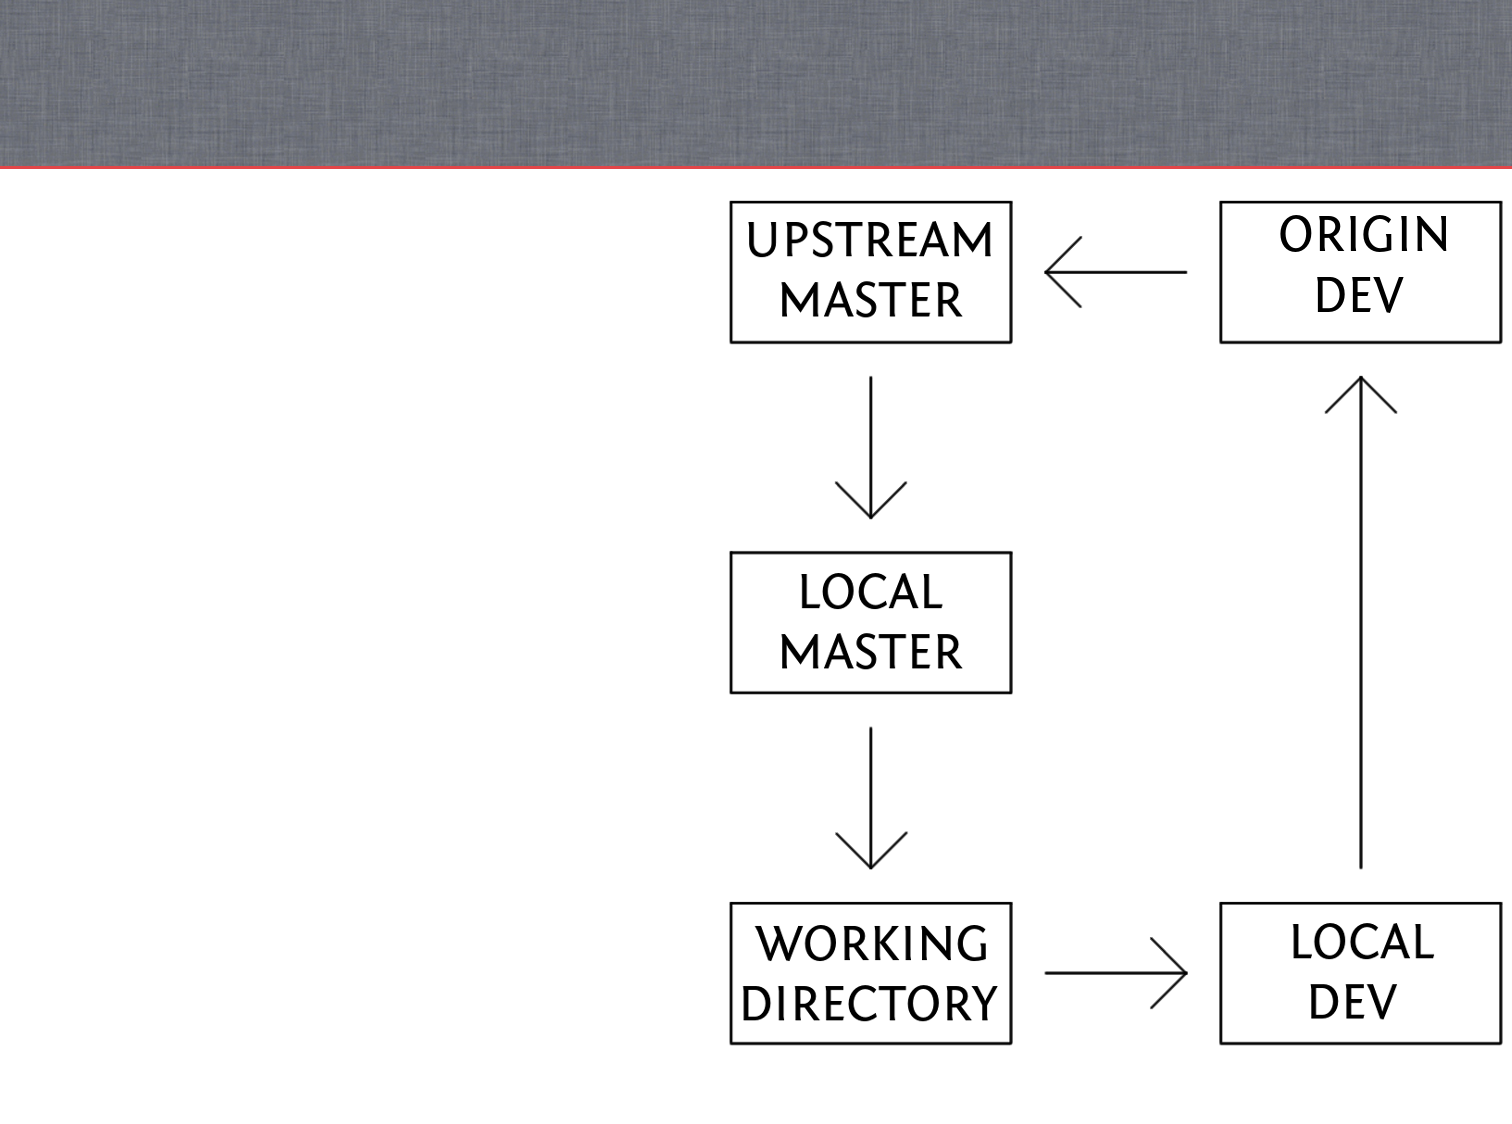
\includegraphics[width=\paperwidth,height=\paperheight]{assets/workflow_bg}}
\begin{frame}
    \vspace{1cm} % generate some space between title and content
    \frametitle{Our Sample Workflow}
        1. Pull from Upstream Master to \\
        Local Master \linebreak\linebreak
        2. Branch to Working Directory \linebreak\linebreak
        3. Make and test changes \linebreak\linebreak
        4. Commit to Local Dev \linebreak\linebreak
        5. Push to Origin Dev \linebreak\linebreak
        6. Open pull request to Upstream \\
        Master
    \vspace{1cm} % generate some space between title and content
\end{frame}
\setbeamertemplate{background}
{
\includegraphics[width=\paperwidth,height=\paperheight]{assets/slide_bg}}

\begin{frame}
    \frametitle{Get source code}
    \begin{itemize}
        \item{sign up for hacktoberfest}
        \item{Fork the repo to which you want to contribute}
        \item{Clone the repo - copies it to your local machine.  ``` git clone <repo html>```}
        \item{Mac: ???}
    \end{itemize}
    \vspace{1cm} % generate some space between title and content
\end{frame}

\end{document}
